\documentclass[11pt,a4paper]{article}

\usepackage[utf8]{inputenc}
\usepackage[T1]{fontenc}
\usepackage[margin=1in]{geometry}
\usepackage{amsmath,amssymb,amsfonts}
\usepackage{graphicx}
\usepackage{xcolor}
\usepackage{booktabs}
\usepackage{tabularx}
\usepackage{array}
\usepackage{listings}
\usepackage{tikz}
\usetikzlibrary{shapes.geometric, arrows.meta, positioning, calc, fit}
\usepackage{enumitem}
\usepackage{caption}
\usepackage{subcaption}
\usepackage{float}
\usepackage{hyperref}

\hypersetup{
    colorlinks=true,
    linkcolor=black,
    citecolor=black,
    urlcolor=blue!70!black,
    pdftitle={SMTP, POP3 and IMAP4 Servers and Clients},
    pdfauthor={Subham Bhat}
}

\definecolor{codebg}{rgb}{0.96,0.96,0.96}
\definecolor{codeframe}{rgb}{0.25,0.25,0.25}
\definecolor{codenum}{rgb}{0.45,0.45,0.45}

\lstset{
    backgroundcolor=\color{codebg},
    basicstyle=\ttfamily\footnotesize,
    breakatwhitespace=false,
    breaklines=true,
    captionpos=b,
    commentstyle=\color{codenum}\itshape,
    keywordstyle=\bfseries,
    numberstyle=\tiny\color{codenum},
    numbers=left,
    numbersep=8pt,
    frame=single,
    rulecolor=\color{codeframe},
    tabsize=4,
    columns=flexible,
    keepspaces=true,
    showspaces=false,
    showstringspaces=false,
    xleftmargin=14pt,
    xrightmargin=4pt,
    literate={→}{{$\rightarrow$}}1 {←}{{$\leftarrow$}}1 {–}{{--}}1 {—}{{---}}1 {·}{{$\cdot$}}1 {✓}{{OK}}2 {✗}{{X}}1
}

\newcolumntype{Y}{>{\raggedright\arraybackslash}X}

% screenshot from docs/screenshots (skipped quietly if the file is missing)
\newcommand{\shot}[3][0.92\textwidth]{%
  \IfFileExists{docs/screenshots/#2}{%
  \begin{figure}[H]\centering
  \includegraphics[width=#1,keepaspectratio]{docs/screenshots/#2}
  \caption{#3}\end{figure}}{}}

\emergencystretch=3em
\setlength{\parindent}{1.5em}
\setlength{\parskip}{0.4em}

\begin{document}

% ==============================================================================
% TITLE PAGE
% ==============================================================================
\begin{titlepage}
    \centering
    \vspace*{4.2cm}

    {\LARGE \textbf{Electronic Mail from the RFCs: SMTP, POP3}}\\[0.7em]
    {\LARGE \textbf{and IMAP4 Servers and Clients, MIME,}}\\[0.7em]
    {\LARGE \textbf{STARTTLS, and Real-Provider Interoperation}}\\[1.4em]

    {\large for Computer Networks Laboratory}

    \vspace{3.8cm}

    {\large
    \textbf{Name:} Subham Bhat\\[0.55em]
    \textbf{Class:} BCSE III\\[0.55em]
    \textbf{Roll:} 002410501020\\[0.55em]
    \textbf{Group:} A1\\[0.55em]
    \textbf{College:} Jadavpur University
    }

    \vfill
    {\normalsize 1}
\end{titlepage}

% ==============================================================================
% TABLE OF CONTENTS
% ==============================================================================
\pagenumbering{roman}
\setcounter{page}{2}
\tableofcontents
\newpage

% ==============================================================================
% MAIN CONTENT
% ==============================================================================
\pagenumbering{arabic}
\setcounter{page}{3}

\section{Introduction}
\noindent Electronic mail is the oldest application on the Internet that is still used by almost everyone. Unlike the web, it is \emph{asynchronous}: the sender and the receiver are rarely online at the same time, so mail is stored on servers between the two. This gives the system two halves with different protocols:
\begin{itemize}[leftmargin=2em]
    \item \textbf{Push:} the user agent hands a message to its mail server, and servers hand it on to each other, with the \textbf{Simple Mail Transfer Protocol} (\textbf{SMTP}, RFC 5321) on TCP port 25 (587 for submission, 465 with implicit TLS).
    \item \textbf{Pull:} the recipient fetches mail from the server with a \emph{mail access protocol}: \textbf{POP3} (RFC 1939, port 110/995), which downloads and usually deletes, or \textbf{IMAP4} (RFC 3501, port 143/993), which keeps mail, folders and flags on the server so that several devices stay in sync.
\end{itemize}
SMTP carries only 7-bit text lines, so attachments and non-English text need \textbf{MIME} (RFC 2045--2047). Because all three protocols were designed as plaintext, each has an extension to upgrade the same connection to TLS (\texttt{STARTTLS}, \texttt{STLS}).

\subsection{What Was Built}
This module implements both sides of e-mail from the RFCs in pure Java 11 with no external libraries:
\begin{enumerate}[leftmargin=2em]
    \item \textbf{An SMTP server} with ESMTP extensions, STARTTLS, AUTH PLAIN/LOGIN, dot-stuffing, \texttt{Received:} headers, relay protection and bounce messages (DSN).
    \item \textbf{A POP3 server} with the AUTHORIZATION $\rightarrow$ TRANSACTION $\rightarrow$ UPDATE state machine, maildrop locking and STLS.
    \item \textbf{An IMAP4rev1 server} with folders, FETCH, STORE, server-side SEARCH, COPY/MOVE, APPEND and \textbf{IDLE} push notifications.
    \item \textbf{SMTP, POP3 and IMAP clients} that work with our servers \emph{and} with real providers (Gmail, Outlook) over TLS.
    \item \textbf{A MIME library}: multipart attachments, base64, quoted-printable and RFC 2047 encoded subjects.
    \item \textbf{An optional smart host}: outside mail can be relayed through a real provider such as Gmail.
    \item \textbf{A live dashboard} on \texttt{http://localhost:8083}: the full protocol conversation with every reply code explained, a POP3 vs IMAP experiment on two devices, a MIME viewer and a raw command console.
\end{enumerate}

\begin{table}[H]
\centering
\caption{Ports used by the Mail module}
\small
\begin{tabularx}{\textwidth}{@{}lccY@{}}
\toprule
\textbf{Protocol} & \textbf{Plain (+STARTTLS)} & \textbf{Implicit TLS} & \textbf{Real-world ports} \\ \midrule
SMTP & 2525 & 2465 & 25, 587 (submission), 465 \\
POP3 & 1110 & 2995 & 110, 995 \\
IMAP & 1143 & 2993 & 143, 993 \\
Dashboard & HTTP 8083 & & \\ \bottomrule
\end{tabularx}
\end{table}

\shot{01_architecture.png}{The architecture section of the dashboard: user agent, SMTP push, mailbox, POP3/IMAP pull, animated by real traffic.}

% ==============================================================================
\section{Protocols and Message Formats}

\subsection{SMTP: Commands, Envelope and Replies}
An SMTP transaction separates the \textbf{envelope} from the \textbf{message}. \texttt{MAIL FROM} and \texttt{RCPT TO} form the envelope: they decide where the message is delivered and where bounces go. The \texttt{From:} and \texttt{To:} lines are only headers inside the message, which is why BCC works.

\begin{lstlisting}[numbers=none, caption={A complete SMTP session with STARTTLS and AUTH (S = server, C = client).}]
S: 220 mail.cse.myuniv.edu ESMTP JU-Mail ready
C: EHLO laptop
S: 250-mail.cse.myuniv.edu Hello laptop [127.0.0.1]
S: 250-SIZE 10485760
S: 250-8BITMIME
S: 250-PIPELINING
S: 250-STARTTLS
S: 250-AUTH PLAIN LOGIN
S: 250-ENHANCEDSTATUSCODES
S: 250 HELP
C: STARTTLS
S: 220 2.0.0 Ready to start TLS          ... TLS handshake on the same TCP connection ...
C: EHLO laptop                           (start over: everything before was plaintext)
C: AUTH PLAIN AGFsaWNlAGFsaWNlMTIz
S: 235 2.7.0 Authentication successful
C: MAIL FROM:<alice@cse.myuniv.edu>
S: 250 2.1.0 Sender <alice@cse.myuniv.edu> OK
C: RCPT TO:<bob@cse.myuniv.edu>
S: 250 2.1.5 Recipient <bob@cse.myuniv.edu> OK
C: DATA
S: 354 End data with <CR><LF>.<CR><LF>
C: Subject: Hello ... (headers, blank line, body) ...
C: .
S: 250 2.0.0 OK: queued as 28DF34898CF8
C: QUIT
S: 221 2.0.0 mail.cse.myuniv.edu closing connection
\end{lstlisting}

\begin{table}[H]
\centering
\caption{SMTP reply-code classes}
\small
\begin{tabularx}{\textwidth}{@{}lY@{}}
\toprule
\textbf{Code} & \textbf{Meaning} \\ \midrule
2xx & Success: 220 ready, 221 closing, 235 authenticated, 250 OK. \\
3xx & Intermediate: 334 AUTH challenge, 354 send the message data. \\
4xx & Transient failure: try again later. \\
5xx & Permanent failure: 535 authentication failed, 550 no such user, 552 too large, 554 relay denied. \\ \bottomrule
\end{tabularx}
\end{table}

\subsection{POP3 and IMAP4}
POP3 has three states. In \textbf{AUTHORIZATION} the client logs in (\texttt{USER}, \texttt{PASS}); in \textbf{TRANSACTION} it lists and retrieves messages (\texttt{STAT}, \texttt{LIST}, \texttt{UIDL}, \texttt{RETR}, \texttt{TOP}) and marks some for deletion (\texttt{DELE}, undone by \texttt{RSET}); only after \texttt{QUIT}, in \textbf{UPDATE}, are the marked messages really removed. POP3 knows nothing about folders or read flags.

IMAP keeps everything on the server. Every command carries a \textbf{tag} so that replies can be matched and several commands can be in flight; untagged responses (\texttt{* 3 EXISTS}) report changes. Flags such as \texttt{\textbackslash Seen} and \texttt{\textbackslash Deleted}, folders, and searches all live on the server, so every device sees the same state.

\subsection{MIME}
A message with an attachment is a \texttt{multipart/mixed} body whose parts are separated by a boundary string. Each part has its own \texttt{Content-Type} and \texttt{Content-Transfer-Encoding}: text is usually \textbf{quoted-printable}, binary data \textbf{base64} (about 33\% larger, because 3 bytes become 4 characters). Non-ASCII header text uses RFC 2047 encoded words such as \texttt{=?UTF-8?B?\ldots?=}.

% ==============================================================================
\section{System Architecture}

\begin{figure}[H]
\centering
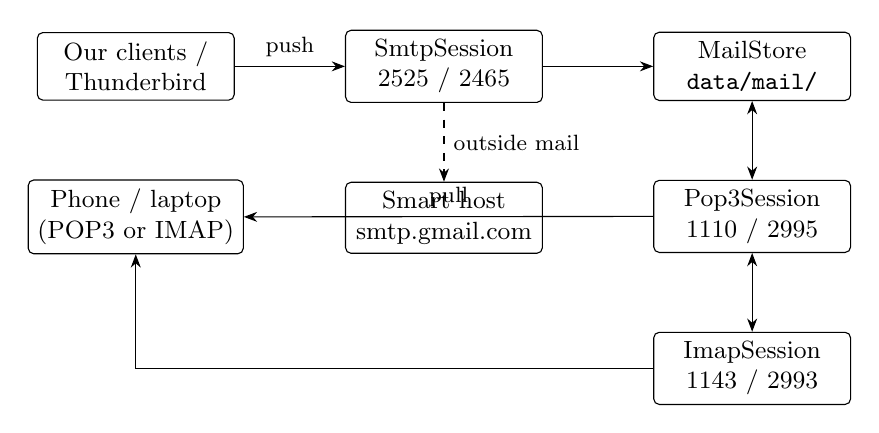
\begin{tikzpicture}[node distance=0.9cm, box/.style={draw, rounded corners=2pt, minimum width=2.5cm, minimum height=0.85cm, align=center, font=\small}, >=Stealth]
\node[box] (ua) {Our clients /\\Thunderbird};
\node[box, right=1.4cm of ua] (smtp) {SmtpSession\\2525 / 2465};
\node[box, right=1.4cm of smtp] (store) {MailStore\\\texttt{data/mail/}};
\node[box, below=1.0cm of store] (pop) {Pop3Session\\1110 / 2995};
\node[box, below=1.0cm of pop] (imap) {ImapSession\\1143 / 2993};
\node[box, below=1.0cm of ua] (dev) {Phone / laptop\\(POP3 or IMAP)};
\node[box, below=1.0cm of smtp] (gm) {Smart host\\smtp.gmail.com};
\draw[->] (ua) -- node[above, font=\footnotesize]{push} (smtp);
\draw[->] (smtp) -- (store);
\draw[<->] (store) -- (pop); \draw[<->] (pop) -- (imap);
\draw[->] (pop.west) -- node[above, font=\footnotesize]{pull} (dev.east);
\draw[->] (imap.west) -| (dev.south);
\draw[->, dashed] (smtp) -- node[right, font=\footnotesize]{outside mail} (gm);
\end{tikzpicture}
\caption{Components of the Mail module.}
\end{figure}

\begin{table}[H]
\centering
\caption{Source packages}
\small
\begin{tabularx}{\textwidth}{@{}lY@{}}
\toprule
\textbf{Package} & \textbf{Responsibility} \\ \midrule
\texttt{server/} & \texttt{Session} (base: listener, one thread per connection, STARTTLS upgrade), \texttt{SmtpSession}, \texttt{Pop3Session}, \texttt{ImapSession}. \\
\texttt{client/} & \texttt{LineClient} (base: plain, STARTTLS, implicit TLS), \texttt{SmtpClient}, \texttt{Pop3Client}, \texttt{ImapClient}. \\
\texttt{store/} & \texttt{MailStore}: one folder per mailbox, one \texttt{.eml} file per message, UIDs and flags. \\
\texttt{mime/} & \texttt{Mime}: build and parse multipart messages, base64, quoted-printable, RFC 2047. \\
\texttt{dashboard/}, \texttt{core/} & HTTP API and the event hub that records every protocol line. \\ \bottomrule
\end{tabularx}
\end{table}

\textbf{TLS.} On first start \texttt{keytool} creates a self-signed certificate (\texttt{data/mail-tls.p12}). For STARTTLS the server answers \texttt{220 Ready}, then wraps the \emph{existing} socket with \texttt{SSLSocketFactory.createSocket(sock, host, port, true)} and performs the handshake. The implicit-TLS ports use an SSL server socket from the start. The clients use the same call in client mode and verify real providers' certificates with Java's default trust store.

% ==============================================================================
\section{Implementation}

\subsection{SMTP Server: Relay Protection, Dot-Stuffing and Bounces}
Recipients in our own domain are accepted only if the user exists (\texttt{550} otherwise). Recipients in other domains are accepted only from an authenticated user; anyone else gets \texttt{554 Relay access denied}, so the server is not an \emph{open relay} that spammers could abuse.

\begin{lstlisting}[language=Java, caption={RCPT handling in \texttt{SmtpSession.java}.}]
private void rcpt(String arg) throws IOException {
    if (from == null) { reply("503 5.5.1 Need MAIL before RCPT"); return; }
    String addr = angle(arg.substring(3).trim());
    int at = addr.indexOf('@');
    String user = at > 0 ? addr.substring(0, at) : addr;
    String dom  = at > 0 ? addr.substring(at + 1) : ctx.store.domain;
    if (dom.equalsIgnoreCase(ctx.store.domain)) {
        if (!ctx.store.userExists(user)) { reply("550 5.1.1 <" + addr + ">: Recipient address rejected: User unknown"); return; }
        local.add(user.toLowerCase(Locale.ROOT));
        reply("250 2.1.5 Recipient <" + addr + "> OK");
    } else if (authUser != null) {
        remote.add(addr);
        reply("250 2.1.5 Recipient <" + addr + "> OK (will relay)");
    } else {
        reply("554 5.7.1 <" + addr + ">: Relay access denied");   // no open relay
    }
}
\end{lstlisting}

The message ends with a line holding only a dot. A body line that itself starts with a dot is sent with an extra dot by the client (\emph{dot-stuffing}) and the server removes it. The server then prepends \texttt{Return-Path:} and \texttt{Received:} headers and files the message in each local INBOX.

\begin{lstlisting}[language=Java, caption={Reading DATA, undoing dot-stuffing and adding trace headers.}]
reply("354 End data with <CR><LF>.<CR><LF>");
while ((l = readLine()) != null) {
    if (l.equals(".")) break;                       // end of message
    if (l.startsWith("..")) l = l.substring(1);      // undo dot-stuffing
    if (body.size() < MAX_SIZE) body.write((l + "\r\n").getBytes(StandardCharsets.UTF_8));
}
String received = "Return-Path: <" + from + ">\r\n"
        + "Received: from " + helo + " (" + peer + ") by mail." + ctx.store.domain + " (JU-Mail) with "
        + (authUser != null ? "E" : "") + "SMTP" + (secure ? "S" : "") + (authUser != null ? "A" : "")
        + " id " + qid + "; " + Mime.rfc822Date(new Date()) + "\r\n";
for (String u : local) ctx.store.append(u, "INBOX", msg, null);
for (String r : remote) relayOrBounce(r, msg, subject);
reply("250 2.0.0 OK: queued as " + qid);
\end{lstlisting}

\textbf{Outside mail.} A real mail server would look up the recipient domain's MX record in DNS and connect to it on port 25. A lab PC cannot do that (ISPs block port 25 and providers reject mail from unknown home addresses), so without further configuration the server writes a \textbf{delivery status notification} back to the sender's INBOX. If \texttt{data/smarthost.properties} names a provider, the server instead logs in to it as a client over STARTTLS with AUTH and hands the message on, exactly as Outlook or Thunderbird sends through Gmail. With a Gmail app password configured, a letter posted from the dashboard was delivered to a real Gmail inbox.

\shot{02_smtp_send_transcript.png}{Sending a letter: the colour-coded transcript with every reply code explained.}

\subsection{POP3: Locking and the UPDATE State}
The maildrop is locked for the whole session, so a second POP3 session for the same user is refused. \texttt{DELE} only records the message number; the deletion happens in the UPDATE state after \texttt{QUIT}.

\begin{lstlisting}[language=Java, caption={The UPDATE state in \texttt{Pop3Session.java}.}]
private void quit() throws IOException {
    if (state == State.TRANSACTION) {
        MailStore.Folder inbox = ctx.store.folder(user, "INBOX");
        for (int n : deleted) {                        // only now are DELE marks applied
            MailStore.Message m = drop.get(n - 1);
            Set<String> f = new TreeSet<>(m.flags);
            f.add("\\Deleted");
            ctx.store.setFlags(user, inbox, m, f);
        }
        int removed = ctx.store.expunge(user, inbox).size();
        ok("Bye: " + removed + " message(s) deleted", "UPDATE state: messages removed, lock released");
    } else ok("Bye", "");
}
\end{lstlisting}

\subsection{IMAP4: Server-Side State and IDLE Push}
The IMAP server supports tags, literals and sequence/UID sets; \texttt{LIST}, \texttt{SELECT}/\texttt{EXAMINE} and \texttt{STATUS}; \texttt{FETCH} of flags, envelope, body structure and partial bodies (with \texttt{BODY.PEEK} that does not set \texttt{\textbackslash Seen}); \texttt{STORE}, \texttt{SEARCH}, \texttt{COPY}/\texttt{MOVE} (UIDPLUS), \texttt{APPEND}, \texttt{EXPUNGE} and folder management. Changes made by one session are reported to the others as untagged \texttt{EXISTS}, \texttt{EXPUNGE} and \texttt{FETCH FLAGS} responses.

With \textbf{IDLE} (RFC 2177) the client stops polling: the server keeps the connection open and pushes changes until the client sends \texttt{DONE}.

\begin{lstlisting}[language=Java, caption={IDLE in \texttt{ImapSession.java}.}]
private void idle(String tag) throws IOException {
    send("+ idling", "server will now push changes in real time; client ends with DONE");
    idling = true;
    Thread w = new Thread(() -> {
        while (idling) {
            try { Thread.sleep(250); sync(true); } catch (Exception e) { return; }   // push * n EXISTS etc.
        }
    }, id + "-idle");
    w.setDaemon(true);
    w.start();
    String l;
    while ((l = readLine()) != null) if (l.equalsIgnoreCase("DONE")) break;
    idling = false;
    tagged(tag, "OK IDLE terminated");
}
\end{lstlisting}

\subsection{The POP3 vs IMAP Experiment}
The dashboard gives Bob two devices, a phone and a laptop, that share one mailbox. Each can use IMAP, POP3 in keep mode, or POP3 in delete mode.

\begin{table}[H]
\centering
\caption{Observed behaviour of the two-device experiment}
\small
\begin{tabularx}{\textwidth}{@{}lY@{}}
\toprule
\textbf{Setting} & \textbf{Result} \\ \midrule
Phone on POP3 (delete), laptop on IMAP & The phone downloads everything and the server column becomes empty; the laptop then sees no mail and the table reports that the devices disagree. \\
Phone on POP3 (keep) & Letters stay on the server; UIDL tells the phone which ones it already has. Read state is not shared. \\
Both on IMAP & Opening a letter on the laptop sets \texttt{\textbackslash Seen} on the server, and the phone shows it as read. Moving to a folder works only with IMAP. \\
IMAP with IDLE & A new letter appears immediately as a pushed \texttt{* n EXISTS}. \\ \bottomrule
\end{tabularx}
\end{table}

\shot{03_pop3_vs_imap.png}{The POP3 vs IMAP experiment: what each protocol does to the mailbox on the server.}

\shot[0.85\textwidth]{04_mailbox_console.png}{Inside the mailbox: folders, UIDs, flags, and the MIME tree of a message with an attachment.}

% ==============================================================================
\section{Experiments, Verification and Results}

\subsection{Running the Module}
\begin{lstlisting}[language=bash, caption={Starting the servers, running the checks, and talking SMTP by hand.}]
cd Mail
run.bat                  # SMTP, POP3, IMAP servers and dashboard (http://localhost:8083)
run.bat --verify         # 39 automated end-to-end checks
python interop_test.py   # Python's smtplib, poplib and imaplib against our servers (20 checks)

telnet localhost 2525    # then: EHLO, MAIL FROM, RCPT TO, DATA, ".", QUIT
\end{lstlisting}

\subsection{Automated Verification}
All \textbf{39 checks} of \texttt{Verify.java} pass. They drive the real servers with the module's own clients:

\begin{table}[H]
\centering
\caption{Selected verification checks (all passed)}
\small
\begin{tabularx}{\textwidth}{@{}Y@{}}
\toprule
\texttt{multipart/mixed} with two parts; the base64 attachment decodes to the original bytes; RFC 2047 subject round-trips \\
EHLO advertises STARTTLS, AUTH, SIZE, 8BITMIME; STARTTLS upgrade, then a new EHLO no longer offers STARTTLS \\
Unauthenticated relay refused (554); unknown local user rejected (550); wrong password gives 535 \\
Dot-stuffing undone; server added \texttt{Return-Path} and \texttt{Received} headers \\
Authenticated user may relay; with no smart host a bounce (DSN) is delivered to the sender \\
POP3: UIDL gives permanent ids; a second session is refused (maildrop locked); DELE only marks, QUIT removes \\
IMAP: \texttt{BODY.PEEK} does not set \texttt{\textbackslash Seen}, \texttt{BODY[]} does; device B sees device A's flag change \\
IMAP IDLE: new mail is pushed to device B; UID MOVE, APPEND to Sent, CREATE folder \\
A POP3 delete on one device shows up as EXPUNGE on the IMAP device \\
SMTPS, POP3S and IMAPS (implicit TLS) and STARTTLS/STLS all work \\ \bottomrule
\end{tabularx}
\end{table}

\subsection{Interoperation}
\begin{enumerate}[leftmargin=2em]
    \item \textbf{Standard libraries against our servers.} \texttt{interop\_test.py} uses Python's \texttt{smtplib}, \texttt{poplib} and \texttt{imaplib}, which we did not write, to send, list, fetch, search and append; all 20 checks pass. This shows the servers follow the RFCs rather than only our own client.
    \item \textbf{Real mail applications.} Thunderbird configured with IMAP \texttt{localhost:1143} and SMTP \texttt{localhost:2525} sends and reads mail; read flags stay in sync with the dashboard.
    \item \textbf{Our clients against real providers.} The dashboard's clients connect to Gmail and Outlook over TLS (IMAP 993, POP3 995, SMTP 587 with STARTTLS) using an app password.
    \item \textbf{Real delivery through a smart host.} With Gmail configured as smart host, a letter posted to an external Gmail address from the dashboard arrived in that Gmail inbox.
\end{enumerate}

\shot[0.85\textwidth]{05_real_provider_compare.png}{The same clients connected to a real provider.}

% ==============================================================================
\section{Conclusion}
\begin{enumerate}[leftmargin=2em]
    \item \textbf{Push and pull are different problems.} SMTP moves mail between servers and must decide whom it may relay for; POP3 and IMAP give a user access to a stored mailbox. Building all three showed why they are separate protocols.
    \item \textbf{Where state lives decides the user experience.} POP3 in delete mode left a second device with nothing; IMAP kept folders and read flags on the server and, with IDLE, pushed new mail without polling.
    \item \textbf{Plaintext protocols can be upgraded in place.} STARTTLS and STLS wrap the existing TCP connection in TLS, after which the session starts over; credentials were never sent before the upgrade.
    \item \textbf{The servers are real.} Python's standard mail libraries, Thunderbird and Windows \texttt{telnet} all work with them, and the same clients work with Gmail, so the implementation follows the RFCs rather than a private convention.
\end{enumerate}

\section*{AI Acknowledgement}
\addcontentsline{toc}{section}{AI Acknowledgement}
Artificial Intelligence tools were used as an aid during this project. Specifically, AI assistance was used for:
\begin{itemize}[leftmargin=2em]
    \item \textbf{Protocol cross-checking:} comparing message formats, reply codes, state machines and byte offsets against the RFCs cited in this report.
    \item \textbf{Code review and testing:} suggesting edge cases for the automated verification suite and reviewing concurrency and error handling.
    \item \textbf{Writing and visualization:} drafting, structuring and refining the explanations, tables, diagrams and \LaTeX{} source of this report.
\end{itemize}
All protocol implementations, Java source code, experiments, measurements and final conclusions were run, reviewed and verified by the author, who takes full responsibility for the content of this report.

\end{document}
